This chapter briefly presents the main characteristics of SDN and the main ML algorithms. For a more in-depth knowledge on ML applied to the SDN refer to \cite{Xie2019}.
\section{Software Defined Networks Architecture} \label{sec:SDN_BGK}
The Open Networking Foundation (ONF) \cite{ONF} is a nonprofit consortium dedicated to the development and standardization of SDN. The SDN paradigm has been defined by ONF as follows: “In the SDN architecture, the control plane and data plane are decoupled, network intelligence and state are logically centralized, and the underlying network infrastructure is abstracted from the applications” \cite{Sezer2013}.
A SDN architecture is composed by three main planes, including data plane, control plane and application plane. The architectural components of each plane and their interactions are shown in Figure \ref{fig:{ONF}}. In the following, we will give a brief description of these planes and their interactions.
\begin{figure}[tb!]
	\centering
	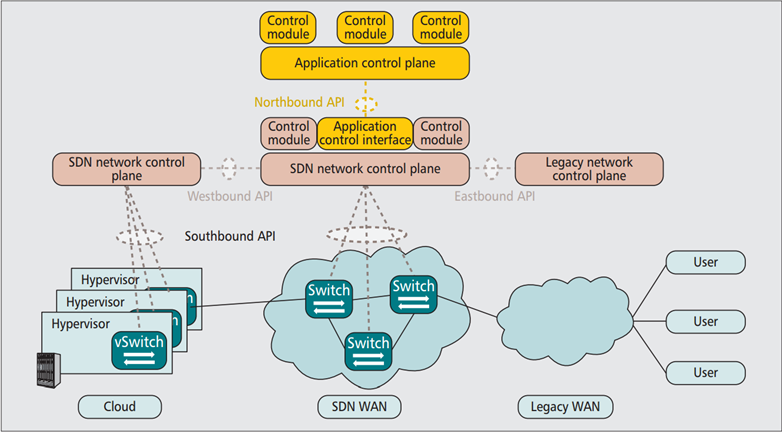
\includegraphics[width=13cm]{figure/ONF.png}
	\caption{The high-level SDN architecture.}
	\label{fig:{ONF}}
\end{figure}
\begin{itemize}
\item[] \textbf{Data Plane} : The data plane, or infrastructure plane, is the lowest layer in SDN architecture. This plane is composed by physical switches and virtual switches and others forwarding devices. Virtual switches are software-based switches, which can run on common operating systems. Open vSwitch \cite{OVS}, Indigo \cite{Indigo} and Pantou \cite{Pantou} are three implementations of virtual switches. Physical switches are hardware-based switches. They can be implemented on open network hardware (e.g., NetFPGA \cite{Lockwood2007}) or implemented on networking hardware vendors’ merchant switches. Many networking hardware vendors such as HP, NEC, Huawei, Juniper and Cisco, have supported SDN protocols. Virtual switches support complete features of SDN protocols, while physical switches lack the flexibility and feature completeness. However, physical switches have a higher flow forwarding rate than virtual switches.  SwitchBlade \cite{Anwer2010} and ServerSwitch \cite{Lu2011} are two NetFPGA-based physical switches.
These switches in data plane are responsible for forwarding, dropping and modifying packets based on instructions received from the Control Plane (CP) through Southbound Interfaces (SBIs).
\item[] \textbf{Control Plane}: The control plane is the “brain” of SDN systems, which can define network resources, dynamically choose forwarding rules and make network administration flexible and agile. The controller is responsable of many relevant tasks like:
\begin{itemize}
\item[•] the communication between forwarding devices and applications;
\item[•] it exposes and abstracts network state information of the data plane to the application plane;
\item[•] it translates the requirements from applications into custom policies and distributes them to forwarding devices;
\item[•] provides essential functionalities that most of network applications need, such as shortest path routing, network topology storage, device configuration and state information notifications etc.
\end{itemize}
There are many controller architectures, such as Ryu \cite{RYU}, OpenDayLight, \cite{Medved2014} NOX \cite{NOX}, POX \cite{POX}, Floodlight \cite{Floodlight} and Beacon \cite{Erickson2013}. Three communication interfaces allow the controllers to interact: southbound, northbound (NBI) and eastbound/westbound interfaces.
The	SBIs are defined between the control plane and the data plane. They allow forwarding devices to exchange network state information and control policies with the CP and provide functions such as statistics reports, forwarding operations, programmatic control of all device-capability advertisements and event notifications. OpenFlow \cite{McKeown2008} promoted by ONF is the first and the most popular open standard SBI. There exist other less popular proposals such as OVSDB \cite{OVS_Pfaff}, Protocol-Oblivious Forwarding (POF) \cite{Song2013} and OpenState \cite{Bianchi2014}. With NBIs, automation, innovation and management of SDN networks has been facilitate thanks to the fact that applications can exploit the abstract network views provided by the CP. The ONF is trying to define the standard NBIs and a common information model.
The eastbound/westbound interfaces are used in the multi-controller SDN networks. Due to the vast amount of data flows in such networks and the limited processing capacity of one controller the large-scale networks are always partitioned into several domains and each domain has its own controller.
The eastbound/westbound interfaces are responsible for the communication among multiple controllers. This communication  is necessary to exchange information in order to provide a global network view to the upper-layer applications. Onix \cite{Koponen} and HyperFlow \cite{Tootoonchian} are two distributed control architectures. Because their eastbound/westbound interfaces are private, they cannot communicate with each other. To enable the communication between different types of SDN controllers, SDNi \cite{yin2012}, East-West Bridge \cite{Lin2013} and Communication Interface for Distributed Control plane (CIDC) \cite{Benamrane2017} have been proposed as eastbound/westbound interfaces to exchange network information. However, the eastbound/westbound interfaces have not yet been standardized.
\item []\textbf{Application Plane}: The highest layer in the SDN architecture is the application plane. These applications can provide new services and perform business management, optimization and can obtain the required network state information through controllers’ NBIs. Based on the received information and other requirements, the applications can apply some control logic to change network behaviors.
The SDN-based applications have attracted a lot of attention from academia. Mendiola et al. \cite{Mendiola2017} have discussed the impact of SDN on Traffic Engineering (TE) and surveyed the SDN-based TE solutions. Security in SDN has been surveyed in \cite{Ahmad2015, ScottHayward2016, Rawat2017, Ali2015, Yan2016, Dargahi2017}. Especially, Yan et al. \cite{Yan2016} have researched on Distributed Denial of Service (DDoS) attacks in SDN-based cloud computing systems, and discussed future research challenges. Fault management in SDN has been surveyed in \cite{Fonseca2017}, which gives an identification and classification of the main fault management issues, and does valuable surveys and discussions about efforts that address those issues. Guck et al. \cite{Guck2018} have studied the centralized QoS routing mechanisms in SDN, and introduced a novel Four-Dimensional (4D) evaluation framework.
SDN has been deployed in many networks, such as transport networks \cite{Alvizu2017}, optical networks \cite{Thyagaturu2016}, wireless networks \cite{Haque2016, Chen2015}, Internet of Things (IoT) \cite{Bera2017}, edge computing \cite{Baktir2017}, Wide Area Networks (WAN) \cite{Michel2017}, cloud computing \cite{Jain2013}, Network Function Virtualization (NFV) \cite{Li2015, Liang2015}.
\end{itemize}
For more informations on SDN, please refer to \cite{Nunes2014, Jarraya2014, Xia2015, Hu2014, Xie2015, Trois2016, Huang2017, Blenk2016}.

%
%\subsection{Workflow}
To understand the SDN architecture, it is important to recall its basic operation. Figure \ref{fig:{WorkFlow}} shows the working procedure of the OpenFlow-based SDN network \cite{OFP13}. Each OpenFlow switch has a flow table and uses the OpenFlow protocol to communicate with the SDN controller. The messages transmitted between the OpenFlow-based switches and the software-based controller are standardized by the OpenFlow protocol \cite{Erickson2013}. The OpenFlow controller can manage the traffic forwarding by modifying flow entries in switches flow tables.
\begin{figure}[tb!]
	\centering
	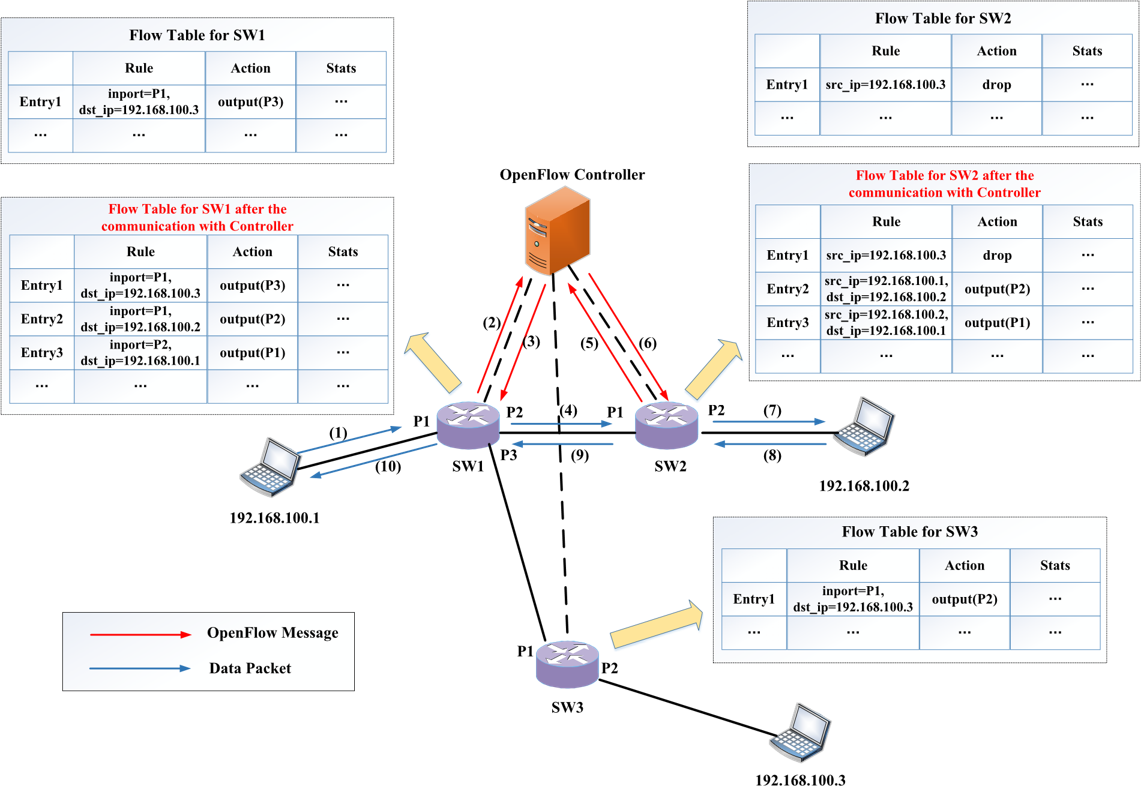
\includegraphics[width=13cm]{figure/WorkFlow.png}
	\caption{Example of OpenFlow-based SDN network.}
	\label{fig:{WorkFlow}}
\end{figure}
The flow table in the OpenFlow switch is comprised of flow entries to determine the processing actions of different packets on the data plane. When an OpenFlow switch receives a packet on the data plane, the packet header fields will be extracted and matched against flow entries. If a matching entry is found, the switch will process the packet locally according to the actions in matched flow entry. Otherwise, the switch will forward an OpenFlow PacketIn message to the controller (arrows 2 and 5). The packet header (or the whole packet, optionally) is included in the OpenFlow PacketIn message. Then, the controller will send OpenFlow FlowMod messages to manage the switch’s flow table by adding flow entries (arrows 3 and 6), which can be used to process subsequent packets of the flow.  For example, by adding two flow entries (i.e., Entry2 and Entry3) at SW1 and SW2, the communications between $192.168.100.1$ and $192.168.100.2$ are allowed.
However, packets from $192.168.100.3$ to $192.168.100.2$ are denied at SW2 due to security policies.
%====================================================================================================
%====================================================================================================